\documentclass[11pt]{article}

\usepackage[margin=1in]{geometry}
\usepackage[T1]{fontenc}
\usepackage{lmodern}
\usepackage{microtype}
\usepackage{amsmath,amssymb,amsthm,mathtools}
\usepackage{mathrsfs}
\usepackage[dvipsnames]{xcolor}
\usepackage[most]{tcolorbox}
\usepackage{tikz}
\usetikzlibrary{decorations.markings}
\usepackage{enumitem}
\usepackage{tocloft}
\usepackage[hidelinks]{hyperref}

\definecolor{courseblue}{HTML}{1F4E79}
\definecolor{lightblue}{HTML}{EAF2F8}
\definecolor{lightgreen}{HTML}{EAF7EA}
\definecolor{lightpink}{HTML}{FCE8EF}
\definecolor{lightyellow}{HTML}{FFF8D6}
\definecolor{warningyellow}{HTML}{D6A000}
\definecolor{exercisebg}{HTML}{D6E6F5}
\definecolor{exerciseframe}{HTML}{1F4E79}
\definecolor{examplebg}{HTML}{F4FAFE}
\definecolor{exampleframe}{HTML}{85C1E9}
\definecolor{darkgray}{HTML}{333333}
\definecolor{lightorange}{HTML}{FDEBD8}
\definecolor{orangeframe}{HTML}{E08A3C}

\setlength{\parindent}{0pt}
\setlength{\parskip}{0.65em}
\setlist[itemize]{topsep=0.25em,itemsep=0.15em}
\renewcommand{\cftsecleader}{\cftdotfill{\cftdotsep}}
\renewcommand{\cftsubsecleader}{\cftdotfill{\cftdotsep}}

\theoremstyle{plain}
\newtheorem{theorem}{Theorem}[section]
\newtheorem{proposition}[theorem]{Proposition}
\newtheorem{lemma}[theorem]{Lemma}
\newtheorem{corollary}[theorem]{Corollary}
\theoremstyle{definition}
\newtheorem{definition}[theorem]{Definition}
\newtheorem{example}[theorem]{Example}
\newtheorem{exercise}[theorem]{Exercise}
\theoremstyle{remark}
\newtheorem*{remark}{Remark}
\newtheorem*{fact}{Fact}
\newtheorem*{warning}{Warning}

\tcolorboxenvironment{definition}{
  enhanced,
  unbreakable,
  colback=lightgreen,
  colframe=ForestGreen,
  boxrule=0.7pt,
  arc=2pt,
  left=6pt,
  right=6pt,
  top=5pt,
  bottom=5pt
}

\tcolorboxenvironment{warning}{
  enhanced,
  colback=lightyellow,
  colframe=warningyellow,
  boxrule=0.7pt,
  arc=2pt,
  left=6pt,
  right=6pt,
  top=5pt,
  bottom=5pt
}

\tcolorboxenvironment{exercise}{
  enhanced,
  colback=exercisebg,
  colframe=exerciseframe,
  boxrule=1pt,
  arc=2pt,
  left=6pt,
  right=6pt,
  top=5pt,
  bottom=5pt
}

\tcolorboxenvironment{example}{
  enhanced,
  colback=examplebg,
  colframe=exampleframe,
  boxrule=0.7pt,
  arc=2pt,
  left=6pt,
  right=6pt,
  top=5pt,
  bottom=5pt
}

\numberwithin{equation}{section}

\newcommand{\be}{\begin{eqnarray}}
\newcommand{\ee}{\end{eqnarray}}
\newcommand{\C}{\mathbb{C}}
\newcommand{\R}{\mathbb{R}}
\newcommand{\N}{\mathbb{N}}

\DeclareMathOperator{\Hol}{\mathcal{H}\mathrm{ol}}
\DeclareMathOperator{\Real}{Re}
\DeclareMathOperator{\Imag}{Im}
\newcommand{\A}{\mathcal{A}}
\newcommand{\CT}{\C[[T]]}
\newcommand{\CLT}{\C((T))}
\tcbset{breakable}
\begin{document}

\begin{center}
  \colorbox{lightblue}{%
    \begin{minipage}{0.94\textwidth}
      \vspace{0.55em}
      \begin{tabular*}{\textwidth}{@{\extracolsep{\fill}}lr}
        {\color{courseblue}\bfseries\LARGE Lecture 16} &
        {\color{courseblue}\bfseries\LARGE MATH 411}\\[0.35em]
        \textbf{Fall 2026} & \textbf{Date: Oct 16, 2026}\\
        & \textbf{Instructor: Manish Patnaik}
      \end{tabular*}
      \vspace{0.45em}
    \end{minipage}}
\end{center}

\setcounter{tocdepth}{1}
\tableofcontents
\vspace{0.45em}

% Sources: handwritten Lecture 15, pages 5--7; Lecture 16, pages 1--7.
In Lecture~15 we established the chain-of-discs lemma for continuous curves.
We now use it to define integrals of holomorphic functions along continuous
curves using local primitives, then preview the local Cauchy integral formula
and introduce homotopy of curves.

\section{Integrating holomorphic functions along continuous curves}
% Continued from Lecture 15, beginning with the definition of partition.
\begin{tcolorbox}[
 enhanced,
 unbreakable,
 colback=lightyellow,
 colframe=warningyellow,
 boxrule=0.7pt,
 arc=2pt,
 left=6pt,
 right=6pt,
 top=5pt,
 bottom=5pt
]
\textbf{Definition (Partition).} Let $\gamma\colon[a,b]\to U$ be
continuous, with $U$ open and $a<b$. Write
\[
 P:=\{a_0,\ldots,a_n\},\qquad a=a_0<\cdots<a_n=b,
\]
for a \emph{subdivision of $[a,b]$}. Using the chain-of-discs lemma
from Lecture~15, we call the data
\[
 \mathscr{D}:=\bigl(P,D_0,\ldots,D_{n-1}\bigr)
\]
a \emph{partition of $\gamma$} if each
$D_j$ is an open disc contained in $U$ with
$\gamma([a_j,a_{j+1}])\subseteq D_j$.
We call $P$ the \emph{underlying subdivision} of $\mathscr{D}$.
\end{tcolorbox}

We recall Lemma~2.4 from Lecture~15, which guarantees that partitions exist.

\begin{lemma}[A chain of discs along a curve]\label{lem:partition-existence}
Let $\gamma\colon[a,b]\to U$ be continuous, with $U$ open and $a<b$.
There exist a subdivision
\[
 a=a_0<a_1<\cdots<a_n=b
\]
and open discs $D_0,\ldots,D_{n-1}\subseteq U$ such that
$\gamma([a_j,a_{j+1}])\subseteq D_j$ for every $j$.
Equivalently, every such curve admits a partition.
\end{lemma}
\begin{proof}
The image $K=\gamma([a,b])$ is compact. By
the uniform-neighbourhood lemma from Lecture~15, choose $r>0$ such that
$D(z,r)\subseteq U$ for every $z\in K$.
Also, $\gamma$ is uniformly continuous on $[a,b]$. Thus there is
$\delta>0$ such that
\[
 s,t\in[a,b],\quad |s-t|<\delta\quad\Longrightarrow\quad
 |\gamma(s)-\gamma(t)|<r/2.
\]
Choose a subdivision with $a_{j+1}-a_j<\delta$, and set
$D_j=D(\gamma(a_j),r)$. For $t\in[a_j,a_{j+1}]$,
$|\gamma(t)-\gamma(a_j)|<r/2$, so the whole subcurve lies in $D_j$.
\end{proof}

\subsection{Definition by local primitives}
\begin{definition}\label{def:continuous-integral}
Let $f$ be holomorphic on an open set $U$, and let
$\gamma\colon[a,b]\to U$ be continuous, with $a\leq b$.
If $a<b$, choose a partition $\mathscr{D}$ as above. On each $D_j$,
choose a primitive $g_j$ of $f$, which exists by Cauchy's theorem on
a disc. Define
\begin{equation}\label{eq:continuous-integral}
 \boxed{\displaystyle
 \int_\gamma f(z)\,dz
 =\sum_{j=0}^{n-1}\left[
 g_j\bigl(\gamma(a_{j+1})\bigr)-g_j\bigl(\gamma(a_j)\bigr)
 \right].}
\end{equation}
If $a=b$, define the integral to be zero.
\end{definition}

\begin{remark}
This definition uses the continuity of the curve and the holomorphicity
of $f$. No derivative of $\gamma$ is needed.
\end{remark}

\begin{proposition}\label{prop:well-defined}
The value in \eqref{eq:continuous-integral} is independent of the
partition $\mathscr{D}$ and the chosen local primitives. For a piecewise
continuously differentiable path, it agrees with the usual contour integral.
\end{proposition}
\begin{proof}
If $a=b$, our definition and the usual contour integral both give zero.
We therefore assume $a<b$.

\textbf{Choice of primitive.} If $g$ and $h$ are primitives of $f$ on
one disc $D$, then $(g-h)'=0$. Since $D$ is connected, $g-h$ is constant.
Consequently, for any $w_0,w_1\in D$,
\[
 g(w_1)-g(w_0)=h(w_1)-h(w_0).
\]

\textbf{Possible changes of partition.}
Recall that $\mathscr{D}$ consists of subdivision points \emph{and}
one disc for each subinterval. There are two basic changes to consider:
\begin{enumerate}
 \item \emph{Insert a subdivision point.} Replace $[a_j,a_{j+1}]$ by
 $[a_j,c]$ and $[c,a_{j+1}]$, where $a_j<c<a_{j+1}$. We may use the
 same disc $D_j$ for both pieces, since both subcurves still lie in $D_j$.
 Repeating this operation is called a \emph{refinement of the subdivision}.
 \item \emph{Change a disc.} Keep the subdivision points fixed and
 replace $D_j$ by another open disc $\widetilde D_j\subseteq U$ containing
 the entire subcurve $\gamma([a_j,a_{j+1}])$. The discs need not contain
 one another; it is enough that both contain this subcurve.
\end{enumerate}
One may also remove or move subdivision points, provided the resulting
data still form a partition of $\gamma$. For example, removing a point
requires a disc in $U$ containing the whole merged subcurve. We will
compare such changes by refining both subdivisions to a common one.

\begin{center}
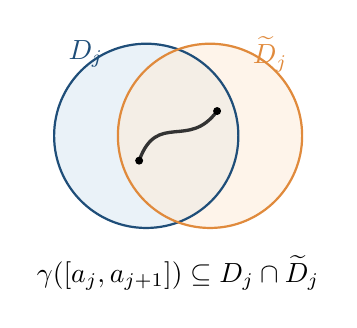
\begin{tikzpicture}[scale=0.9]
 \fill[lightblue] (-0.45,0) circle (1.3);
 \fill[lightorange,fill opacity=0.55] (0.45,0) circle (1.3);
 \draw[thick,courseblue] (-0.45,0) circle (1.3);
 \draw[thick,orangeframe] (0.45,0) circle (1.3);
 \draw[very thick,darkgray] (-0.55,-0.35)
 .. controls (-0.3,0.35) and (0.15,-0.2) .. (0.55,0.35);
 \fill (-0.55,-0.35) circle (1.6pt);
 \fill (0.55,0.35) circle (1.6pt);
 \node[courseblue] at (-1.3,1.15){$D_j$};
 \node[orangeframe] at (1.3,1.15){$\widetilde D_j$};
 \node[below] at (0,-1.55)
 {$\gamma([a_j,a_{j+1}])\subseteq D_j\cap\widetilde D_j$};
\end{tikzpicture}
\end{center}

\textbf{What is a common refinement?}
Given two subdivisions $P=\{a_0,\ldots,a_n\}$ and
$Q=\{b_0,\ldots,b_m\}$ of $[a,b]$, list all their points in increasing
order, counting a point only once if it occurs in both:
\[
 P\cup Q=\{s_0,\ldots,s_N\},\qquad a=s_0<\cdots<s_N=b.
\]
This is their \emph{common refinement}: it is obtained from either
subdivision by inserting points. Each new subinterval
$[s_k,s_{k+1}]$ lies in one subinterval of $P$ and one of $Q$.

\begin{center}
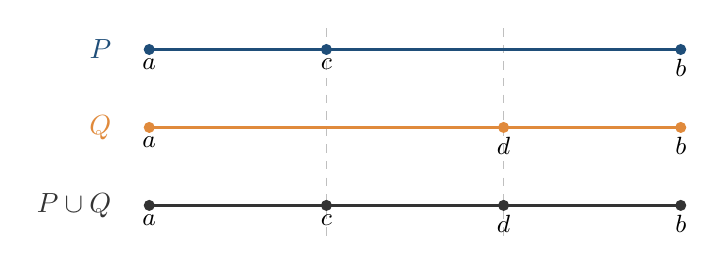
\begin{tikzpicture}[x=0.9cm,y=0.9cm]
 \draw[gray!50,dashed] (2.5,0.3)--(2.5,-2.65);
 \draw[gray!50,dashed] (5,0.3)--(5,-2.65);
 \draw[thick,courseblue] (0,0)--(7.5,0);
 \draw[thick,orangeframe] (0,-1.1)--(7.5,-1.1);
 \draw[thick,darkgray] (0,-2.2)--(7.5,-2.2);
 \node[left,courseblue] at (-0.4,0){$P$};
 \node[left,orangeframe] at (-0.4,-1.1){$Q$};
 \node[left,darkgray] at (-0.4,-2.2){$P\cup Q$};
 \foreach \x/\lab in {0/a,2.5/c,7.5/b}
 {\fill[courseblue] (\x,0) circle (2pt);
  \node[below,font=\small] at (\x,0){$\lab$};}
 \foreach \x/\lab in {0/a,5/d,7.5/b}
 {\fill[orangeframe] (\x,-1.1) circle (2pt);
  \node[below,font=\small] at (\x,-1.1){$\lab$};}
 \foreach \x/\lab in {0/a,2.5/c,5/d,7.5/b}
 {\fill[darkgray] (\x,-2.2) circle (2pt);
  \node[below,font=\small] at (\x,-2.2){$\lab$};}
\end{tikzpicture}
\end{center}

The common refinement aligns the subdivision points; it does not yet
make the disc choices identical. Refine each partition by retaining
its own original disc on every smaller piece. Thus each new subcurve
lies in both an inherited disc $D_j$ from the first partition and an
inherited disc $\widetilde D_\ell$ from the second:
\[
 \gamma([s_k,s_{k+1}])\subseteq D_j\cap\widetilde D_\ell.
\]
We can therefore compare the two primitive increments on this intersection.

\textbf{Refinement of the partition.}
We now check that the changes just described preserve the defining sum.
Insert $c\in(a_j,a_{j+1})$, keeping the disc $D_j$ and its primitive
$g_j$ on both new pieces. Write
\[
 u=\gamma(a_j),\qquad v=\gamma(c),\qquad w=\gamma(a_{j+1}).
\]
The old contribution is $g_j(w)-g_j(u)$, whereas the two new
contributions add to
\begin{align*}
 [g_j(v)-g_j(u)]+[g_j(w)-g_j(v)]
 &=g_j(w)-g_j(u).
\end{align*}
The two values at the inserted point cancel. All other terms in the
sum are unchanged, so inserting one point preserves the sum. By
repeating this argument, any finite refinement preserves it. If we
choose different primitives on the new pieces, the first part of the
proof shows that their endpoint differences are the same.

\begin{center}
\begin{minipage}[t]{0.48\linewidth}
\centering
\vspace{0pt}
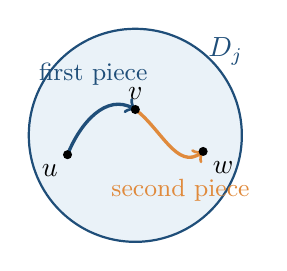
\begin{tikzpicture}[scale=0.82]
 \fill[lightblue] (0,0) circle (1.65);
 \draw[thick,courseblue] (0,0) circle (1.65);
 \node[courseblue] at (1.4,1.3){$D_j$};
 \draw[very thick,courseblue,->] (-1.05,-0.3)
 .. controls (-0.85,0.2) and (-0.45,0.65) .. (0,0.4);
 \draw[very thick,orangeframe,->] (0,0.4)
 .. controls (0.4,0.1) and (0.65,-0.55) .. (1.05,-0.25);
 \fill (-1.05,-0.3) circle (2pt) node[below left]{$u$};
 \fill (0,0.4) circle (2pt) node[above]{$v$};
 \fill (1.05,-0.25) circle (2pt) node[below right]{$w$};
 \node[courseblue,font=\small] at (-0.65,0.95){first piece};
 \node[orangeframe,font=\small] at (0.7,-0.85){second piece};
\end{tikzpicture}
\par\smallskip
{\small One disc and one primitive: the value at $v$ cancels.\par}
\end{minipage}\hfill
\begin{minipage}[t]{0.48\linewidth}
\centering
\vspace{0pt}
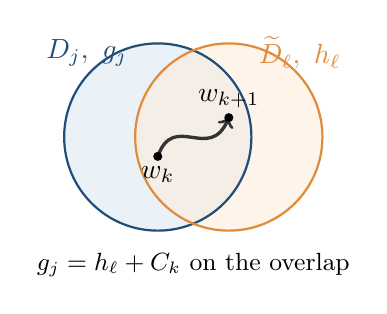
\begin{tikzpicture}[scale=0.82]
 \fill[lightblue] (-0.55,0) circle (1.45);
 \fill[lightorange,fill opacity=0.55] (0.55,0) circle (1.45);
 \draw[thick,courseblue] (-0.55,0) circle (1.45);
 \draw[thick,orangeframe] (0.55,0) circle (1.45);
 \node[courseblue] at (-1.65,1.3){$D_j,\ g_j$};
 \node[orangeframe] at (1.65,1.3){$\widetilde D_\ell,\ h_\ell$};
 \draw[very thick,darkgray,->] (-0.55,-0.3)
 .. controls (-0.3,0.4) and (0.25,-0.4) .. (0.55,0.3);
 \fill (-0.55,-0.3) circle (2pt) node[below]{$w_k$};
 \fill (0.55,0.3) circle (2pt) node[above]{$w_{k+1}$};
 \node[below,font=\small] at (0,-1.65){$g_j=h_\ell+C_k$ on the overlap};
\end{tikzpicture}
\par\smallskip
{\small Two discs: the same constant occurs at both endpoints and cancels.\par}
\end{minipage}
\end{center}

\textbf{Choice of discs and partition.}
Consider any two partitions $\mathscr D$ and $\widetilde{\mathscr D}$,
with subdivisions $P$ and $Q$ and primitives $g_j$ on $D_j$ and
$h_\ell$ on $\widetilde D_\ell$. Refine both to
$P\cup Q=\{s_0,\ldots,s_N\}$, retaining their respective discs and
primitives on each smaller piece. The preceding argument shows that
neither sum changes.

Fix one new subinterval $[s_k,s_{k+1}]$, as in the right-hand diagram
above. It lies in an original
subinterval from each partition, so its image lies in
$D_j\cap\widetilde D_\ell$ for suitable $j$ and $\ell$. This
intersection is nonempty, open, and convex, hence connected. On it,
\[
 (g_j-h_\ell)'=f-f=0,
 \qquad\text{so}\qquad g_j-h_\ell=C_k
\]
for a constant $C_k$. Set $w_k=\gamma(s_k)$ and
$w_{k+1}=\gamma(s_{k+1})$. Both endpoints lie in the intersection,
and therefore
\begin{align*}
 g_j(w_{k+1})-g_j(w_k)
 &=[h_\ell(w_{k+1})+C_k]-[h_\ell(w_k)+C_k]\\
 &=h_\ell(w_{k+1})-h_\ell(w_k).
\end{align*}
Thus the two refined sums agree term by term. Since refinement
preserved each original sum, the original sums agree as well. This
proves independence of the partition, including its disc choices.

\textbf{Agreement with the usual integral.}
Suppose now that $\gamma$ is piecewise continuously differentiable.
Start with any partition used in our definition and insert all the
breakpoints of $\gamma$. The defining sum is unchanged. Denote the
refined subdivision by $a=t_0<\cdots<t_M=b$, and let $G_k$ be the
inherited primitive on a disc containing $\gamma([t_k,t_{k+1}])$.

On each of these pieces, the usual fundamental theorem for a
primitive applies:
\[
 \int_{\gamma|_{[t_k,t_{k+1}]}} f(z)\,dz
 =G_k(\gamma(t_{k+1}))-G_k(\gamma(t_k)).
\]
\begin{center}
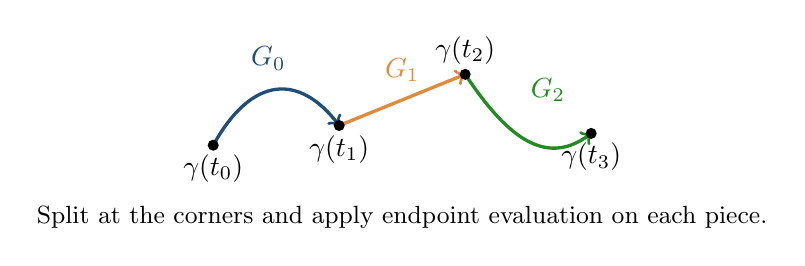
\begin{tikzpicture}[x=1cm,y=1cm]
 \draw[very thick,courseblue,->] (0,0)
 .. controls (0.5,0.9) and (1.1,0.9) .. (1.6,0.25);
 \draw[very thick,orangeframe,->] (1.6,0.25)--(3.2,0.9);
 \draw[very thick,ForestGreen,->] (3.2,0.9)
 .. controls (3.7,0.15) and (4.2,-0.3) .. (4.8,0.15);
 \fill (0,0) circle (2pt) node[below]{$\gamma(t_0)$};
 \fill (1.6,0.25) circle (2pt) node[below]{$\gamma(t_1)$};
 \fill (3.2,0.9) circle (2pt) node[above]{$\gamma(t_2)$};
 \fill (4.8,0.15) circle (2pt) node[below]{$\gamma(t_3)$};
 \node[courseblue] at (0.7,1.1){$G_0$};
 \node[orangeframe] at (2.4,0.95){$G_1$};
 \node[ForestGreen] at (4.25,0.7){$G_2$};
 \node[below,font=\small] at (2.4,-0.65)
 {Split at the corners and apply endpoint evaluation on each piece.};
\end{tikzpicture}
\end{center}
Adding these identities, additivity of the usual contour integral
shows that it equals our defining sum.
\end{proof}

\begin{corollary}[Endpoint evaluation]
If $f$ has a primitive $g$ on $U$, then for every continuous curve
$\gamma\colon[a,b]\to U$,
\[
 \int_\gamma f(z)\,dz=g(\gamma(b))-g(\gamma(a)).
\]
In particular, the integral is zero on every closed continuous curve in
$U$. Thus Cauchy's theorem on a disc also holds for continuous curves.
\end{corollary}
\begin{proof}
Use the restrictions of $g$ as the local primitives. The sum telescopes.
\end{proof}
The integral is linear in $f$, additive when curves are concatenated,
and changes sign when the orientation is reversed. Each property follows
directly from the endpoint differences in \eqref{eq:continuous-integral}.

\section{The local Cauchy integral formula: a preview}
% Handwritten Lecture 16, pages 3--5.
Why do we need integration over continuous curves? One reason is that
we want to deform contours continuously. Here is an important application;
the contour-deformation step will be justified by the homotopy theorem
in the next lecture.

\begin{theorem}[Local Cauchy integral formula]\label{thm:cauchy-formula}
Let $D=D(c,R)$ be an open disc, let $U$ be an open set containing
$\overline D$, and let $f$ be holomorphic on $U$.
If $z_0\in D$ and $\gamma$ is the counterclockwise boundary circle
of $D$, then
\begin{equation}\label{eq:cauchy-formula}
 \boxed{\displaystyle
 f(z_0)=\frac{1}{2\pi i}\int_\gamma\frac{f(z)}{z-z_0}\,dz.}
\end{equation}
\end{theorem}

\begin{proof}[Proof sketch, assuming contour deformation]
For $z\neq z_0$, set
\[
 q(z)=\frac{f(z)-f(z_0)}{z-z_0}.
\]
This is holomorphic on $U\setminus\{z_0\}$. The existence of $f'(z_0)$
gives
\[
 \lim_{z\to z_0}q(z)=f'(z_0),
\]
so $q$ is bounded near $z_0$. We only need this bound; we do not yet
need to prove that the extension of $q$ at $z_0$ is holomorphic.

Choose $0<r<R-|z_0-c|$, and let
$C_r(\theta)=z_0+re^{i\theta}$, $0\leq\theta\leq2\pi$, oriented
counterclockwise. The boundary circle $\gamma$ can be continuously
 deformed to $C_r$ inside $U\setminus\{z_0\}$. The contour-deformation
 theorem, to be proved later, gives
\begin{equation}\label{eq:deformation-preview}
 \int_\gamma q(z)\,dz=\int_{C_r}q(z)\,dz.
\end{equation}

\begin{center}
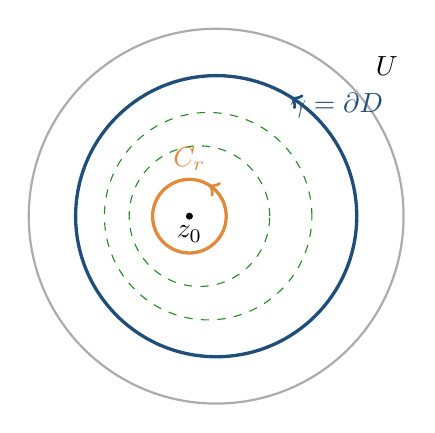
\begin{tikzpicture}[scale=0.85,
 decoration={markings,mark=at position 0.16 with {\arrow{>}}}]
 \draw[thick,gray!65] (0,0) circle (2.8);
 \node at (2.55,2.25){$U$};
 \draw[very thick,courseblue,postaction={decorate}] (2.1,0)
 arc[start angle=0,end angle=360,radius=2.1];
 \fill (-0.4,0) circle (1.5pt) node[below]{$z_0$};
 \draw[very thick,orangeframe,postaction={decorate}] (0.15,0)
 arc[start angle=0,end angle=360,radius=0.55];
 \draw[ForestGreen,dashed] (-0.25,0) circle (1.05);
 \draw[ForestGreen,dashed] (-0.12,0) circle (1.55);
 \node[courseblue] at (1.8,1.65){$\gamma=\partial D$};
 \node[orangeframe] at (-0.4,0.85){$C_r$};
\end{tikzpicture}
\end{center}

Take $M$ such that $|q(z)|\leq M$ near $z_0$. For sufficiently small
$r$, the ML estimate gives
\[
 \left|\int_{C_r}q(z)\,dz\right|\leq2\pi rM\longrightarrow0.
\]
The left side of \eqref{eq:deformation-preview} is independent of $r$,
so $\int_\gamma q=0$. Therefore
\[
 \int_\gamma\frac{f(z)}{z-z_0}\,dz
 =f(z_0)\int_\gamma\frac{dz}{z-z_0}.
\]
Apply the same contour deformation to $1/(z-z_0)$ and parametrize $C_r$:
\[
 \int_\gamma\frac{dz}{z-z_0}
 =\int_{C_r}\frac{dz}{z-z_0}
 =\int_0^{2\pi}\frac{ire^{i\theta}}{re^{i\theta}}\,d\theta
 =2\pi i.
\]
This gives \eqref{eq:cauchy-formula}.
\end{proof}

\begin{remark}
The deformation above is a deformation through \emph{closed curves}:
their common start and end point is allowed to move. Below we first
 define homotopy with fixed endpoints; the closed-curve version and
invariance of integrals will be treated in the next lecture.
\end{remark}

\section{Homotopy of curves}
% Handwritten Lecture 16, pages 5--7.
\subsection{Continuous deformation with fixed endpoints}
\begin{definition}\label{def:homotopy}
Let $\gamma,\eta\colon[a,b]\to U$ be continuous curves with the same
endpoints:
\[
 \gamma(a)=\eta(a),\qquad \gamma(b)=\eta(b).
\]
A \emph{homotopy with fixed endpoints} from $\gamma$ to $\eta$ in $U$
is a continuous map
\[
 H\colon[a,b]\times[0,1]\longrightarrow U
\]
satisfying
\begin{align*}
 H(t,0)&=\gamma(t),& H(t,1)&=\eta(t)&& (a\leq t\leq b),\\
 H(a,s)&=\gamma(a)=\eta(a),&
 H(b,s)&=\gamma(b)=\eta(b)&& (0\leq s\leq1).
\end{align*}
When such an $H$ exists, the curves are \emph{homotopic with fixed
endpoints in $U$}.
\end{definition}
For each fixed $s$, the map $t\mapsto H(t,s)$ is a continuous curve
with the same endpoints. As $s$ runs from $0$ to $1$, these curves
 deform $\gamma$ into $\eta$, staying inside $U$ throughout.

\begin{center}
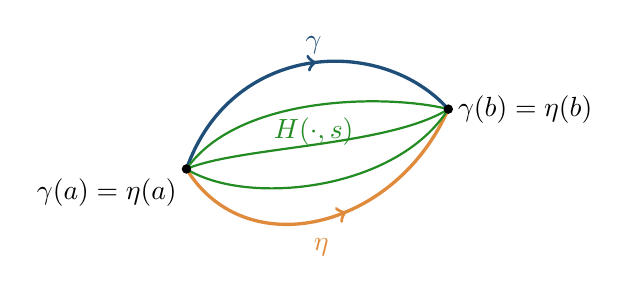
\begin{tikzpicture}[scale=0.95,
 decoration={markings,mark=at position 0.55 with {\arrow{>}}}]
 \draw[very thick,courseblue,postaction={decorate}] (0,0)
 .. controls (0.6,1.7) and (2.6,1.8) .. (3.5,0.8);
 \draw[very thick,orangeframe,postaction={decorate}] (0,0)
 .. controls (0.8,-1.3) and (2.8,-0.8) .. (3.5,0.8);
 \draw[ForestGreen,thick] (0,0) .. controls (0.7,1) and (2.7,1) .. (3.5,0.8);
 \draw[ForestGreen,thick] (0,0) .. controls (0.7,0.3) and (2.7,0.3) .. (3.5,0.8);
 \draw[ForestGreen,thick] (0,0) .. controls (0.8,-0.5) and (2.8,-0.3) .. (3.5,0.8);
 \fill (0,0) circle (1.8pt) node[below left]{$\gamma(a)=\eta(a)$};
 \fill (3.5,0.8) circle (1.8pt) node[right]{$\gamma(b)=\eta(b)$};
 \node[courseblue] at (1.7,1.65){$\gamma$};
 \node[orangeframe] at (1.8,-1.05){$\eta$};
 \node[ForestGreen] at (1.7,0.5){$H(\cdot,s)$};
\end{tikzpicture}
\end{center}

\subsection{Example: curves in a convex set}
\begin{definition}
A set $S\subseteq\C$ is \emph{convex} if, for every $z,w\in S$,
the line segment
\[
 [z,w]=\{(1-s)z+sw:0\leq s\leq1\}
\]
lies in $S$.
\end{definition}
Discs, half-planes, and filled triangles are convex. A region with an
inward notch need not be convex: a segment joining two of its points
 can pass outside the region.

\begin{example}[Straight-line homotopy]
Let $S$ be convex, and let $\gamma,\eta\colon[a,b]\to S$ be continuous
curves with the same endpoints. Define
\begin{equation}\label{eq:straight-homotopy}
 H(t,s)=(1-s)\gamma(t)+s\eta(t).
\end{equation}
This map is continuous, and convexity ensures that $H(t,s)\in S$.
Moreover,
\[
 H(t,0)=\gamma(t),\qquad H(t,1)=\eta(t),
\]
and the endpoints stay fixed because the endpoints of $\gamma$ and
$\eta$ agree. Thus any two such curves in a convex set are homotopic
with fixed endpoints.
\end{example}
In particular, every curve in a convex set can be deformed, keeping its
endpoints fixed, to the straight segment joining those endpoints.
The next step is to prove that integrating a holomorphic function is
invariant under homotopy, and then to justify the contour deformation
used in the Cauchy integral formula.

\end{document}
